\documentclass[11pt,a4paper]{article}

\usepackage[margin=2.4cm]{geometry}
\usepackage{graphicx}
\usepackage{booktabs}
\usepackage{xcolor}
\usepackage{caption}
\usepackage{enumitem}
\usepackage{amsmath}
\usepackage{amssymb}
\usepackage[T1]{fontenc}
\usepackage{lmodern}
\usepackage[colorlinks=true,linkcolor=black,urlcolor=blue,citecolor=black]{hyperref}

\captionsetup{font=small,labelfont=bf}
\setlist{itemsep=2pt,parsep=0pt,topsep=3pt}

% Long identifiers in \code{} are unbreakable and push into the margin; allow
% TeX extra stretch and let \code contents break after underscores.
\emergencystretch=3em
\newcommand{\code}[1]{\texttt{\small\hyphenchar\font=`\-\relax #1}}

\title{\textbf{Sketch-Prompted VLA}\\[2pt]
\large Circle-and-Arrow Disambiguation: Scene-Synthesis Method\\
and Three LIBERO Validation Suites}
\author{Aaron}
\date{28 July 2026}

\begin{document}
\maketitle

\begin{abstract}
\noindent
Natural-language instructions for robot manipulation are frequently ambiguous:
``pick up the bowl and put it on the plate'' does not identify \emph{which} bowl
when four identical bowls are on the table. This project proposes resolving it with
a \textbf{sketch prompt} --- a circle drawn around the intended object and an
arrow pointing at the intended destination, both drawn directly on the robot's
camera view. This report describes the method I use to synthesise validation
scenes for that hypothesis, and the three suites I have built with it on
LIBERO-Spatial, LIBERO-Object and LIBERO-Goal: \textbf{114 scenes} that are
ambiguous \emph{by construction} and machine-scorable. Each scene ships the BDDL
task definition that certifies it, so a trained policy can be scored on it
automatically. The headline text-only versus text+sketch comparison is not
reported here; it requires a trained policy on a GPU. What is reported is the
benchmark those rollouts will run against, and the evidence that it measures
what it claims to.
\end{abstract}

\section{Problem and approach}

A vision-language-action (VLA) policy receives an image and a caption. When the
caption underdetermines the task, the policy cannot succeed reliably --- not
because its manipulation is poor, but because the instruction does not contain
the answer. Existing manipulation benchmarks largely avoid this: their scenes
usually contain exactly one plausible referent, so caption ambiguity never binds.

My claim is that a \textbf{sketch} is a natural and low-bandwidth way for
a human to supply the missing information. A circle says \emph{which object}; an
arrow says \emph{where it goes}. Both are drawn in image space, so they require
no object names, no coordinate frames, and no shared vocabulary between human and
robot.

Testing that claim requires scenes where the sketch is not merely helpful but
\textbf{necessary}. If a scene is solvable from the caption alone, it cannot
discriminate between a policy that reads sketches and one that ignores them. The
core contribution of this work is a scene-synthesis method that produces such
scenes and \emph{proves}, per scene, that they have this property.

\begin{figure}[t]
\centering
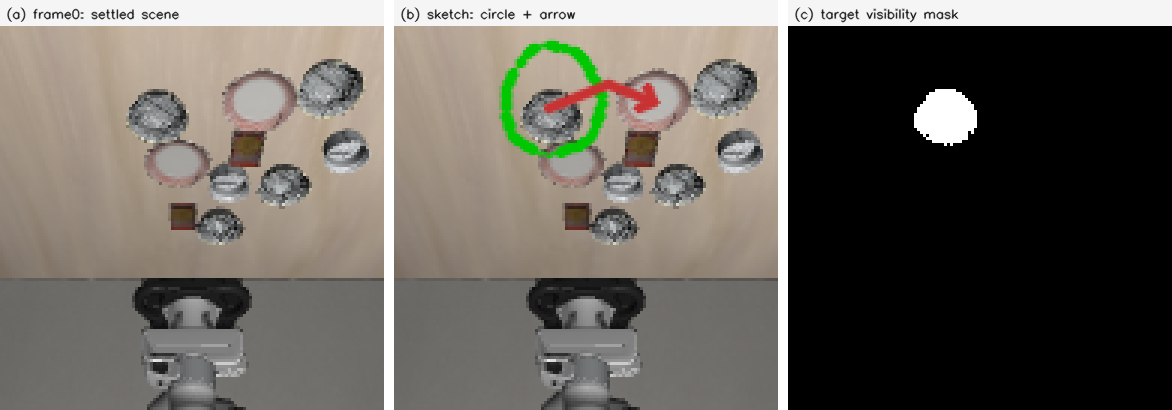
\includegraphics[width=\textwidth]{figures/fig_annotation.png}
\caption{The three artefacts each scene ships (LIBERO-Spatial, \code{scene\_0030}).
(a) the settled scene as the robot sees it, $128\times128$ \code{agentview};
(b) the same frame with the auto-drawn sketch prompt --- a hand-styled circle on
the target and an arrow to the destination; (c) the RGB-difference visibility
mask used to verify the target is actually visible, not occluded behind another
object. Four near-identical bowls are present: the caption alone cannot say which
one to move.}
\label{fig:annotation}
\end{figure}

\section{Scene-synthesis method}

The pipeline is deliberately \emph{generative rather than curated}. I author
LIBERO task definitions as text, instantiate them in the real simulator, measure
the result, and discard anything that fails a gate. Nothing is hand-placed and
nothing is accepted on inspection.

\subsection{Pipeline}

\begin{enumerate}[label=\arabic*.]
\item \textbf{Author the BDDL as text.} LIBERO tasks are declared in BDDL (a
  PDDL-style language) specifying objects, fixtures, placement regions, an
  initial state, and a goal predicate. I write this file by direct string
  templating, injecting duplicate object instances to create the ambiguity and
  retargeting the \code{(:goal)} to one specific instance.
\item \textbf{Instantiate and settle.} The BDDL is loaded with LIBERO's
  \code{OffScreenRenderEnv} and stepped with zero action until the physics
  settles, so recorded poses are resting poses rather than spawn poses.
\item \textbf{Render and project.} I capture the $128\times128$ \code{agentview}
  frame and project every object's ground-truth world position into pixel
  coordinates using the scene's camera matrix, which is stored per scene.
\item \textbf{Draw the sketch.} A circle is drawn around the target's projected
  centre and an arrow from target to destination, both with hand-style jitter so
  the prompt resembles a human annotation rather than a clean overlay.
\item \textbf{Gate.} The scene must pass every check in
  Section~\ref{sec:gates}. A failure discards the scene and \emph{restarts}
  sampling with a fresh seed.
\item \textbf{Package.} The scene folder is written with its BDDL, frames,
  tokens and full provenance.
\end{enumerate}

Every scene records the seed that produced it and is exactly reproducible from
it.

\subsection{The ambiguity tiers}

Ambiguity has two independent axes, and I vary them separately so a failure can
be attributed. Each suite contains the same 38-scene tier distribution.

\begin{table}[h]
\centering
\small
\begin{tabular}{llll}
\toprule
\textbf{Tier} & \textbf{Scenes} & \textbf{Configuration} & \textbf{What is ambiguous} \\
\midrule
control     & 5  & 1 target, 1 destination   & nothing; caption alone suffices \\
referential & 12 & $N$ targets, 1 destination & \emph{which object} \\
directional & 9  & 1 target, $M$ destinations & \emph{which destination} \\
both        & 12 & $N$ targets, $M$ destinations & both axes simultaneously \\
\bottomrule
\end{tabular}
\caption{Tier design, identical across all three suites (38 scenes each).
The \emph{control} tier is the internal sanity check: a policy that fails there
has a manipulation problem, not a disambiguation problem.}
\label{tab:tiers}
\end{table}

\begin{figure}[t]
\centering
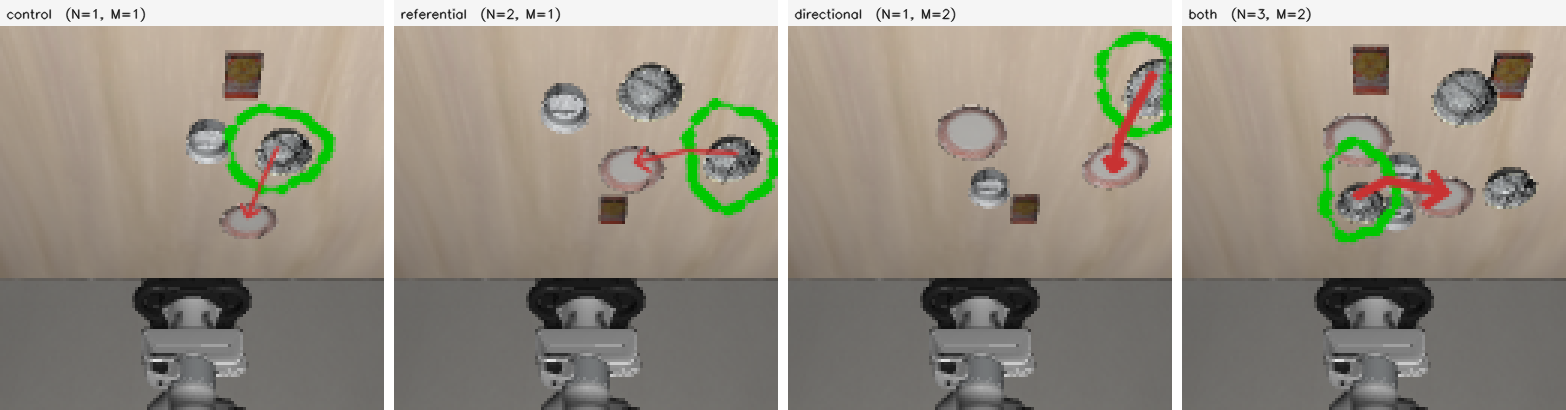
\includegraphics[width=\textwidth]{figures/fig_tiers.png}
\caption{The four tiers, LIBERO-Spatial. $N$ = candidate targets, $M$ =
candidate destinations. Left to right the caption becomes progressively less
sufficient, while the sketch remains equally informative throughout.}
\label{fig:tiers}
\end{figure}

\subsection{The gate stack}
\label{sec:gates}

A scene is kept only if it passes all of the following. The two negative oracles
are the load-bearing ones --- they are what turn ``I believe this scene is
ambiguous'' into ``I have verified this scene is ambiguous''.

\begin{itemize}
\item \textbf{Settled} --- every body rests above the floor plane; nothing has
  fallen through or is still in motion.
\item \textbf{In frame} --- target and all candidate destinations project inside
  the image. A sketch cannot point at something off-screen.
\item \textbf{Visibility $\geq 0.35$} --- the target's unoccluded fraction,
  measured by RGB difference against a frame rendered without it. Segmentation
  masks were tried first and returned empty; the RGB-difference method is what
  works.
\item \textbf{Not pre-solved} --- \code{check\_success()} is \code{False} at
  $t=0$, so the goal is not already satisfied by the initial layout.
\item \textbf{Pixel separation (sketch resolvability)} --- candidates must be far
  enough apart in \emph{image space} for a drawn circle or arrow to distinguish
  them. Thresholds derive from the projected extents of the objects being told
  apart, not from a constant: the circle needs
  $\mathrm{dist}(\text{target},\text{sibling}) \geq r_{\text{drawn}} +
  \mathrm{ext}(\text{sibling}) + 3\,\text{px}$. A constant threshold was wrong
  here, because it scales with the circle while the ambiguity scales with the
  \emph{sibling}.
\item \textbf{Positive oracle} --- teleporting the target to the named
  destination makes the BDDL goal evaluate \code{True}. This proves the scene is
  solvable and that the goal I shipped is the goal I meant.
\item \textbf{Negative oracle, directional} --- moving the target to
  \emph{every other} candidate destination must evaluate \code{False}.
\item \textbf{Negative oracle, referential} --- moving \emph{every} same-category
  sibling to the named destination must evaluate \code{False}.
\item \textbf{Graspable} --- a scripted top-down grasp lifts the target more than
  3\,cm. Enforced in Spatial and Object; recorded but not enforced in Goal, for
  reasons set out in Section~\ref{sec:grasp}.
\end{itemize}

\paragraph{Why the negative oracles matter.}
LIBERO's \code{On(a,b)} predicate is true when $a$ is within 3\,cm in $xy$ of $b$
\emph{and} in contact. Two destination plates placed closer than roughly 6\,cm
therefore both satisfy the goal --- the ``wrong'' answer scores as correct, and
the scene silently stops being a test of anything. The directional negative
oracle catches exactly this case, which no amount of visual inspection would
have revealed.

\paragraph{Design principle.}
Where possible I \emph{satisfy a gate by construction rather than by
rejection}: sampling is constrained so that valid scenes are produced directly,
with rejection as a safety net rather than the primary mechanism. This is why
rejection counts (Table~\ref{tab:suites}) are modest despite the number of gates.

\section{The three suites}

\begin{figure}[h]
\centering
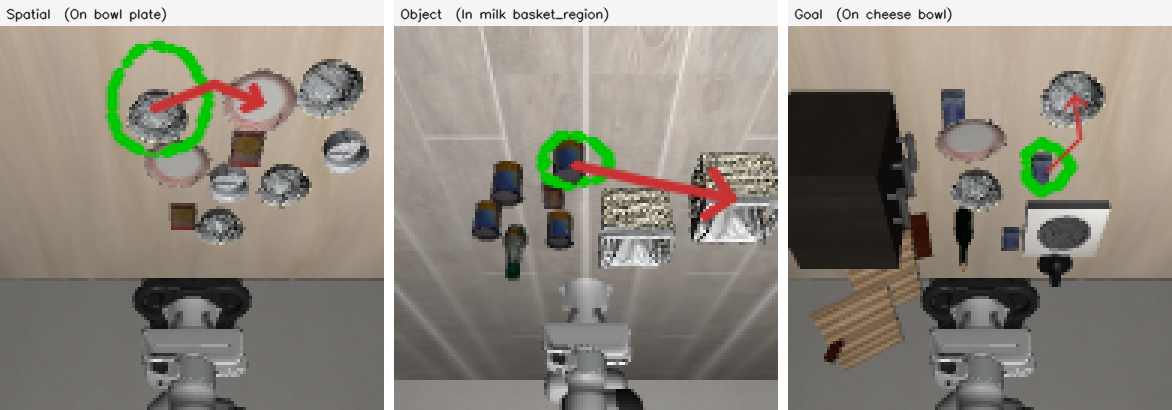
\includegraphics[width=\textwidth]{figures/fig_suites.png}
\caption{One scene from each suite. The suites differ in workspace, predicate
and destination type, but share the tier design, the gate stack and the output
schema.}
\label{fig:suites}
\end{figure}

\subsection{Spatial}

Built from LIBERO-Spatial's tabletop pick-and-place. Goal predicate is
\code{(On bowl\_t plate\_d)}: the destination is an object instance, so
\code{destination\_region} equals \code{destination}. Ambiguity is created by
duplicating black bowls (targets) and plates (destinations). Captions are
degraded to remove the spatial relation that would otherwise disambiguate ---
``pick up the black bowl and place it on the plate''.

\subsection{Object}

Built from LIBERO-Object, where a grocery item is placed \emph{into} a basket.
Goal predicate is \code{(In milk\_t basket\_d\_contain\_region)}: the destination
is a \emph{container region}, so \code{destination} (the basket) and
\code{destination\_region} (its contain region) differ --- a distinction the
schema records explicitly. Ten grocery categories appear as targets, led by
\code{tomato\_sauce} ($\times 6$), \code{alphabet\_soup} ($\times 5$) and
\code{butter} ($\times 5$).

Two facts shaped this suite. Container regions must be \emph{declared} per
basket via \code{(contain\_region (:target basket\_k))}, or the environment
raises \code{KeyError} on the first step. And object size caps how many identical
copies fit the workspace: tall bottles allow at most 3, compact goods 5.

\subsection{Goal}

Built from LIBERO-Goal, which is structurally different from its siblings: there
is no single flat workspace. Each task ships a bespoke scene with real fixtures
(\code{wooden\_cabinet}, \code{flat\_stove}, \code{wine\_rack}) and affordance
regions. The builder therefore \textbf{starts from the original shipped BDDL and
injects} duplicates, preserving every fixture, region and \code{(:init)} line,
and retargeting only the goal.

The decisive property is that a Goal destination is either an \emph{object
instance} (duplicable, so directional and both tiers are possible) or a
\emph{fixed affordance region} (not duplicable). A probe measured the split as 2
object-destination against 6 region-destination tasks. I therefore build all
tasks into control and referential tiers, and the 2 object-destination tasks
additionally into directional and both. One task --- placing a bowl in a drawer
--- was dropped after all 24 candidate seeds failed the positive oracle: the
drawer starts closed, so its region site is retracted and no placement satisfies
the goal. Opening then inserting is two actions, which a single circle-and-arrow
cannot express. The final roster is 7 tasks, all using \code{On}.

\subsection{Comparison}

\begin{table}[h]
\centering
\small
\begin{tabular}{lccc}
\toprule
 & \textbf{Spatial} & \textbf{Object} & \textbf{Goal} \\
\midrule
Scenes                  & 38 & 38 & 38 \\
Goal predicate          & \code{On} & \code{In} & \code{On} \\
Destination type        & object instance & container region & object or region \\
Workspace               & table & floor (banded) & per-task, with fixtures \\
Tasks covered           & 1 & 1 & 7 \\
\midrule
Visibility              & 0.963 / 0.999 / 1.025 & 0.619 / 0.976 / 1.000 & 0.652 / 0.988 / 1.005 \\
Grasp lift (m)          & 0.140 / 0.161 / 0.166 & 0.118 / 0.154 / 0.167 & 0.000 / 0.142 / 0.167 \\
Clearance $xy$ (m)      & 0.086 / 0.136 / 0.245 & 0.110 / 0.160 / 0.326 & 0.079 / 0.160 / 0.396 \\
Px sep., siblings       & 24.1 / 34.2 / 49.5 & 10.6 / 19.5 / 32.4 & 14.6 / 29.9 / 60.9 \\
Px sep., destinations   & 22.4 / 35.0 / 49.0 & 19.1 / 29.4 / 46.9 & 15.5 / 32.4 / 54.1 \\
\midrule
Positive oracle         & 38/38 & 38/38 & 38/38 \\
Grasp succeeded         & 38/38 & 38/38 & \textbf{32/38} \\
Rejections during build & 13 & 30 & 17 \\
\bottomrule
\end{tabular}
\caption{The three suites. Distributions are min / mean / max across the 38
scenes. Pixel separations are reported over the scenes where the corresponding
ambiguity exists ($n=24$ for siblings, $n=21$ for destinations). The single
divergence --- Goal's grasp column --- is the subject of
Section~\ref{sec:grasp}.}
\label{tab:suites}
\end{table}

\section{Output schema and packaging}

All three suites conform to one canonical schema (v1.0), so a single loader and
a single evaluation harness read every scene. Each scene folder contains its
BDDL, the clean frame, the sketch frame, the visibility mask, a model-facing
\code{tokens.json} and a full-provenance \code{meta.json}.

The canonical fields present in every scene are: \code{schema\_version},
\code{suite}, \code{tier}, \code{target}, \code{destination},
\code{destination\_region}, \code{goal\_predicate}, \code{instruction},
\code{symbolic\_tokens} (circle and arrow geometry in pixels), \code{pick\_px},
\code{place\_px}, \code{radius}, \code{camera\_matrix}, \code{visibility},
\code{grasp}, \code{clearance\_xy}, \code{seed} and \code{oracle\_success}.

\paragraph{Two consumer-facing subtleties.}
First, \code{destination\_region} is the exact second argument of the BDDL goal
and is \emph{not} always the destination instance --- for Object it is
\code{basket\_2\_contain\_region} while the destination is \code{basket\_2}. A
scorer must compare against \code{destination\_region}; a renderer wanting the
physical object should use \code{destination}. Second, the combined manifest
\code{validation\_manifest\_all.json} must be keyed on the pair
\code{(suite, dir)}: each suite numbers its scenes from \code{scene\_0000}, so
directory names collide across suites, and seeds overlap as well.

Each suite additionally ships \code{DATASHEET.md}, a \code{contact\_sheet.png}
overview of all 38 scenes, its build log, and both the legacy and canonical
manifests.

\section{The grasp gate: a deliberate divergence in Goal}
\label{sec:grasp}

Spatial and Object \emph{reject} a scene when the scripted top-down grasp fails.
Goal records the result and keeps the scene. Six of its 38 scenes therefore carry
\code{grasp\_success: False}. This was a deliberate decision and is worth stating
plainly, because it affects how Goal results must be reported.

\begin{table}[h]
\centering
\small
\begin{tabular}{lccc}
\toprule
\textbf{Target category} & \textbf{Scenes} & \textbf{Grasp succeeded} & \textbf{Grasp failed} \\
\midrule
\code{akita\_black\_bowl} & 19 & 19 & 0 \\
\code{cream\_cheese}      & 13 & 13 & 0 \\
\code{wine\_bottle}       & 4  & 0  & 4 \\
\code{plate}              & 2  & 0  & 2 \\
\bottomrule
\end{tabular}
\caption{Goal suite, grasp outcome by target category. The split is perfectly
categorical: zero within-category variance.}
\label{tab:grasp}
\end{table}

\paragraph{Why not simply gate it.}
Table~\ref{tab:grasp} shows the failure is a property of the \emph{object
category} under a scripted top-down gripper, not of any particular sampled
placement --- resampling the seed cannot fix it. Contrast the Object suite, whose
15 \code{ungraspable} rejections were all graspable grocery categories in
unlucky placements, which resampling did fix. The same gate therefore does
different work in the two suites: in Object it filters bad samples, whereas in
Goal it would filter nothing and instead delete the \code{wine\_on\_rack},
\code{wine\_on\_cabinet} and \code{plate\_to\_stove\_front} tasks outright,
taking the suite from 7 usable tasks to 4.

What certifies a scene is the positive oracle --- teleporting the target to the
named destination scores the goal \code{True} --- and that is independent of the
scripted grasp. All 38 Goal scenes pass it.

\paragraph{Consequence for scoring.}
A policy that cannot physically lift a wine bottle will score near zero on those
six scenes in \emph{both} the text-only and the text+sketch condition. The
comparison remains valid, since both arms face identical physical difficulty, but
the floor effect compresses the measured effect size and could mask a real
difference. \textbf{Results on the Goal suite should therefore be stratified}:
the headline number over the 32 grasp-succeeding scenes, with the remaining six
reported separately as a manipulation-limited subset. Filter on
\code{meta['grasp']['grasp\_success']}; those scenes are flagged \code{g!} on the
contact sheet.

One caveat on the caveat: a lift of 0.02\,m is a statement about \emph{my
scripted} top-down approach, not about the task's ceiling. A trained policy may
well grasp a wine bottle where the scripted oracle cannot, so this should be
re-examined once GPU rollouts exist rather than assumed permanent.

\section{Verification}

Build-time gates are not trusted on their own; the suites are re-verified
independently after the fact. \code{scripts/audit\_validation\_sets.py} is
read-only and re-parses every \code{scene.bddl} goal predicate directly from
disk, checking it against the canonical \code{target},
\code{destination\_region} and \code{goal\_predicate} recorded in
\code{meta.json} and \code{tokens.json}. It also checks per-scene file
completeness, the full canonical field contract, suite-level packaging, the
\code{(suite, dir)} uniqueness rule, and agreement between the combined manifest
and what is actually on disk.

Current status: \textbf{clean across all 114 scenes, zero mismatches}.

This audit has already earned its keep. It caught 38 Object scenes whose
\code{meta.json} carried the caption under the legacy key \code{language} but
lacked the canonical \code{instruction} field --- a latent fault that would have
raised \code{KeyError} in any harness following the schema, on a third of the
corpus.

\section{Limitations}

\begin{itemize}
\item \textbf{Ambiguity is multiplicity, not occlusion.} The \code{agentview}
  camera looks down steeply, so objects rarely occlude one another and the
  visibility gate seldom binds. Scenes are hard because there are many identical
  candidates, not because the view is cluttered. This corpus should not be cited
  as evidence about occlusion robustness.
\item \textbf{Sketches are synthetic.} Circles and arrows are auto-drawn from
  ground-truth projections with hand-style jitter. Whether humans draw in the
  same places is an open question and an obvious next experiment.
\item \textbf{Goal's harder tiers rest on two tasks.} Only
  \code{bowl\_on\_plate} and \code{cheese\_in\_bowl} have duplicable object
  destinations, so the directional and both tiers derive entirely from them.
\item \textbf{\code{In} is permissive.} Its containment box reaches the floor, so
  an object merely standing at a basket's $xy$ position counts as contained. The
  positive oracle is consequently a weak check in the Object suite; the negative
  oracles carry the weight.
\item \textbf{Long-horizon tasks are excluded.} LIBERO-10 requires two or three
  predicates per goal, which a single circle-and-arrow cannot express. It remains
  postponed rather than solved.
\item \textbf{No policy results yet.} Everything reported here concerns the
  benchmark, not performance on it.
\end{itemize}

\section{Reproduction and next steps}

Each builder runs in WSL2 under a conda environment with
\code{robosuite}, \code{mujoco} and \code{libero}:

\begin{quote}\small
\code{python scripts/build\_validation\_set\_spatial\.py} \\
\code{python scripts/build\_validation\_set\_object\.py} \\
\code{python scripts/build\_validation\_set\_goal\.py} \\
\code{python scripts/package\_goal\_suite.py} \\
\code{python scripts/normalize\_validation\_schema.py} \\
\code{python scripts/audit\_validation\_sets.py}
\end{quote}

The last three need no simulator. Note that re-running a builder resamples and
overwrites that suite's 38 scenes.

\paragraph{Next.}
The immediate blocker is hardware: the text-only versus text+sketch comparison
needs a trained policy on a GPU, which the current 4\,GB laptop cannot host. Once
that exists, the priorities are (i) score all 114 scenes in both conditions,
stratifying Goal by grasp; (ii) run a human-agreement study on sketch placement;
and (iii) export the corpus to RLDS for UniVLA training, which would require
downloading LIBERO-Object and LIBERO-Goal demonstrations, as only Spatial
demonstrations were ever fetched.

\vspace{1em}
\hrule
\vspace{0.6em}
\noindent\small\textbf{Contact sheets.} Every scene in all three suites is shown
on the following page. Tile labels give tier, the $N \times M$ candidate counts,
and measured visibility; Goal tiles additionally give the task name and mark
grasp failures with \code{g!}.

\clearpage
\appendix
\section{Contact sheets}

\begin{figure}[h!]
\centering
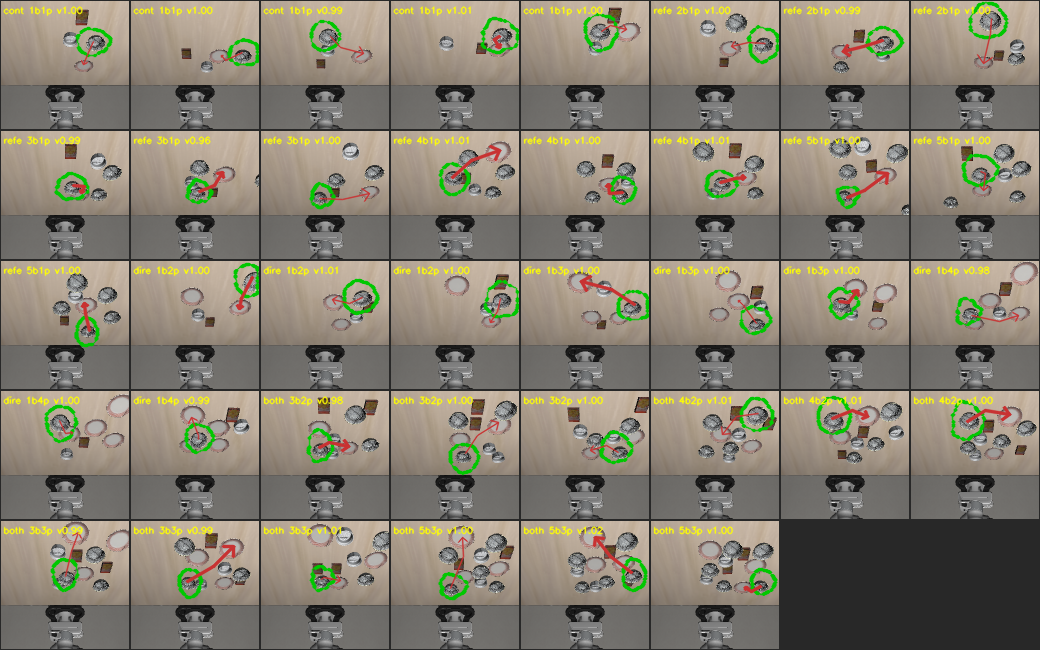
\includegraphics[width=0.86\textwidth]{figures/sheet_spatial.png}
\caption{LIBERO-Spatial, 38 scenes.}
\end{figure}

\begin{figure}[h!]
\centering
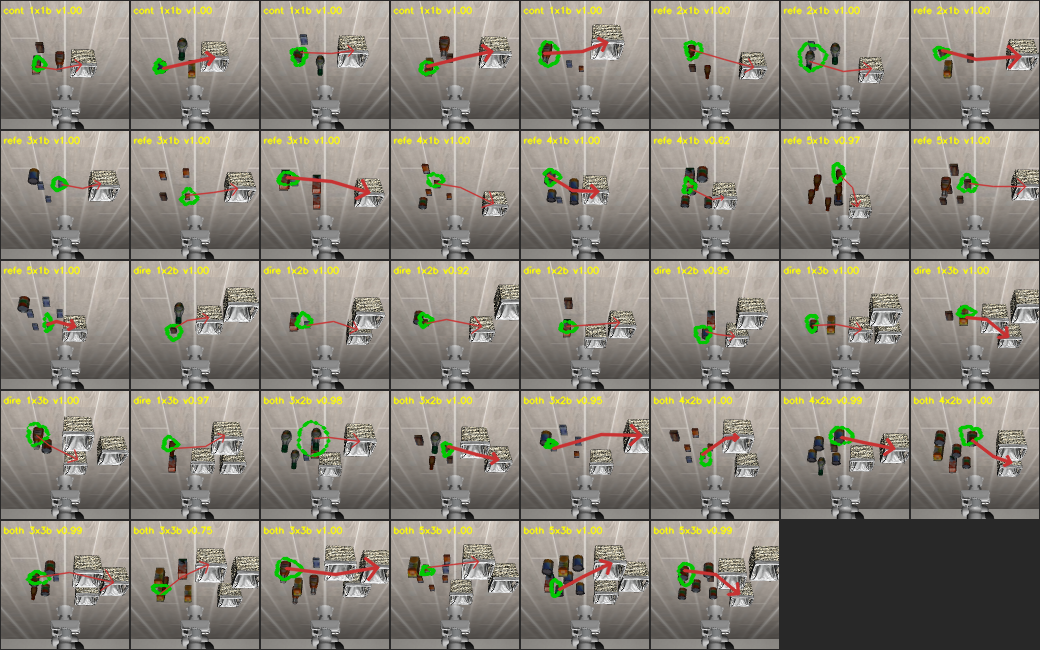
\includegraphics[width=0.86\textwidth]{figures/sheet_object.png}
\caption{LIBERO-Object, 38 scenes.}
\end{figure}

\begin{figure}[h!]
\centering
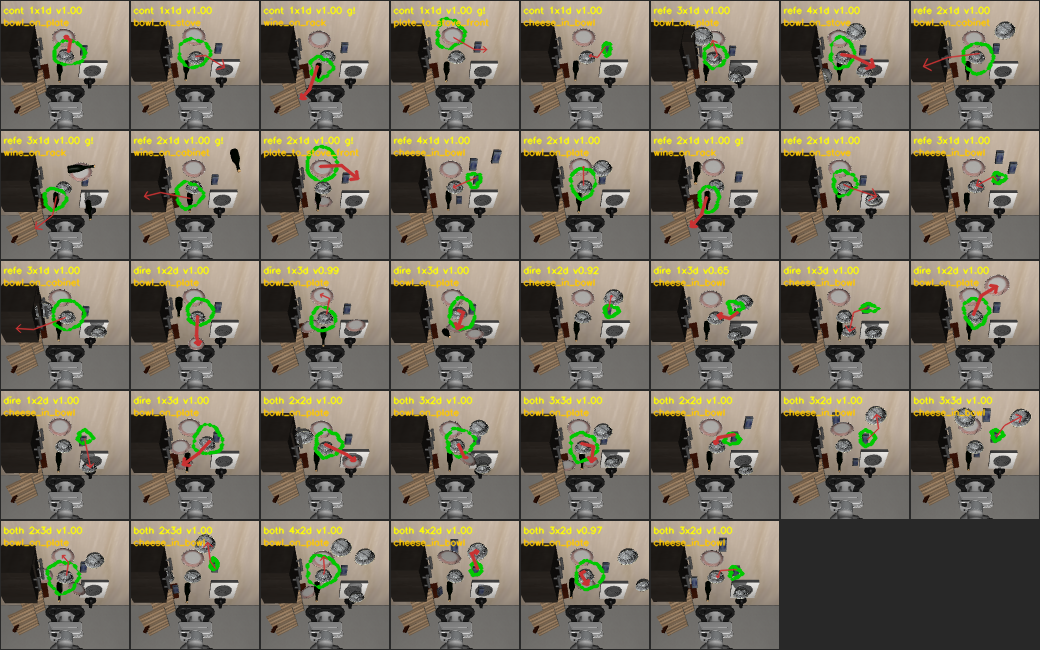
\includegraphics[width=0.86\textwidth]{figures/sheet_goal.png}
\caption{LIBERO-Goal, 38 scenes. Tiles marked \code{g!} are the six scenes
where the scripted grasp fails (Section~\ref{sec:grasp}).}
\end{figure}

\end{document}
